% Foliensatz: "AFu-Kurs nach DJ4UF" von DK0TU, Amateurfunkgruppe der TU Berlin
% Lizenz: CC BY-NC-SA 3.0 de (http://creativecommons.org/licenses/by-nc-sa/3.0/de/)
% Autoren:
% Felix Baum DB4UM <baum@campus.tu-berlin.de>
% Korrekturen:
% Lars Weiler DC4LW <dc4lw@darc.de>

\documentclass[aspectratio=169]{beamer}

\usepackage[ngerman]{babel} % deutsche Worttrennung etc.
\usepackage[utf8]{inputenc} % UTF8 Text

\usepackage[super, comma, numbers, square, sort]{natbib}

\usepackage{hyperref}       % Hyperref Package für bessere Referenzen (todo)
\hypersetup{
	colorlinks=false,       %   false: boxed links; true: colored links
    %linkcolor=white,       %   color of internal links (change box color with linkbordercolor)
    citecolor=red,          %   color of links to bibliography
    filecolor=white,        %   color of file links
    urlcolor=blue           %   color of external links
}

\usepackage{multirow}
\usepackage{wasysym}  % Math Symbols like \permil
%\usepackage{colortbl}
%\usepackage{subscript}
%\usepackage{caption}
%\usepackage{setspace}
%\usepackage{xcolor}        % benutze CodeListe

% Footnote
%\usepackage{hanging}
%
%\setbeamertemplate{footnote}{%
%  \hangpara{2em}{1}%
%  \makebox[2em][l]{\insertfootnotemark}\footnotesize\insertfootnotetext\par%
%}


%\usepackage{pgf}
%\usepackage{tikz}
%\usetikzlibrary{arrows,automata}
%\usetikzlibrary{positioning}
%
%\tikzset{
%    state/.style={
%           rectangle,
%           rounded corners,
%           draw=black, very thick,
%           minimum height=2em,
%           minimum width=2pt,
%           inner sep=2pt,
%           text centered,
%           },
%}

%\usepackage{listings}
%\lstset{basicstyle=\small, numberstyle=\tiny, extendedchars=true, numbers=left, numbersep=5pt}
%\lstset{showtabs=false, showspaces=false, showstringspaces=false}
%%\lstset{backgroundcolor=\color{white!75!lightgray}, , frame=single}
%%\lstset{backgroundcolor=\color{white}}
%%\lstset{backgroundcolor=none}
%\lstset{keywordstyle=\color{blue!50!gray},  identifierstyle=\color{black}}
%\lstset{commentstyle=\color{green!50!gray}, stringstyle=\color{red!50!gray}}
%\lstset{language=C, fontadjust=true, tabsize=2, breaklines=true}
%\lstset{backgroundcolor=\color{white!75!lightgray}, caption=\lstname, frame=single}
%\lstset{emphstyle=\color{black}\fbox}
%
%% Keine "Listing:"-Caption
%\captionsetup{labelformat=empty,labelsep=none}
%
%% für mathematische Umgebungen
%\usepackage{amsmath,amsfonts,amssymb}
%
%\lstdefinestyle{Bash}{
%language=Bash,
%frame=single,
%rulecolor=\color{black},
%backgroundcolor=\color{gray!50},
%keywordstyle=\color{black},
%identifierstyle=,
%commentstyle=\color{black},
%stringstyle=\color{magenta!65!white},
%showstringspaces=false,
%basicstyle=\footnotesize\ttfamily\color{black},
%numbers=none,
%breaklines=true,
%captionpos=b
%}

%\usepackage{listings}
%
%\lstdefinestyle{basic}{
%    captionpos=t,%
%    basicstyle=\footnotesize\ttfamily,%
%    numberstyle=\tiny,%
%    numbers=left,%
%    stepnumber=1,%
%    frame=single,%
%    showspaces=false,%
%    showstringspaces=false,%
%    showtabs=false,%
%    %
%    keywordstyle=\color{blue},%
%    identifierstyle=,%
%    commentstyle=\color{gray},%
%    stringstyle=\color{magenta}%
%}



% fließende Boxen haben keinen Abstand
%\fboxsep0mm

% inkludiere Creative Commons Helper
%%%%%%%%%%%%%%%%%%%%%%%%%%%%%%%%%%%%%%%%%%%%%%%%%%%%%%%%%%%%%%%%
%% ccBeamer 0.1, 2007-07-02                                   %%
%% Written by Sebastian Pipping <webmaster@hartwork.org>      %%
%% ---------------------------------------------------------- %%
%% Licensed under Creative Commons Attribution-ShareAlike 3.0 %%
%% http://creativecommons.org/licenses/by-sa/3.0/             %%
%%%%%%%%%%%%%%%%%%%%%%%%%%%%%%%%%%%%%%%%%%%%%%%%%%%%%%%%%%%%%%%%


%% Images
\newcommand{\CcImageBy}[1]{%
	
\includegraphics[scale=#1]{texdata/creative_commons/cc_by_30.pdf}%
}
\newcommand{\CcImageCc}[1]{%
	
\includegraphics[scale=#1]{texdata/creative_commons/cc_cc_30.pdf}%
}
\newcommand{\CcImageDevNations}[1]{%
	
\includegraphics[scale=#1]{texdata/creative_commons/cc_dev_nations_30.pdf}%
}
\newcommand{\CcImageNc}[1]{%
	
\includegraphics[scale=#1]{texdata/creative_commons/cc_nc_30.pdf}%
}
\newcommand{\CcImageNd}[1]{%
	
\includegraphics[scale=#1]{texdata/creative_commons/cc_nd_30.pdf}%
}
\newcommand{\CcImagePd}[1]{%
	
\includegraphics[scale=#1]{texdata/creative_commons/cc_pd_30.pdf}%
}
\newcommand{\CcImageSa}[1]{%
	
\includegraphics[scale=#1]{texdata/creative_commons/cc_sa_30.pdf}%
}
\newcommand{\CcImageSampling}[1]{%
	
\includegraphics[scale=#1]{texdata/creative_commons/cc_sampling_30.pdf}%
}
\newcommand{\CcImageSamplingPlus}[1]{%
	
\includegraphics[scale=#1]{texdata/creative_commons/cc_sampling_plus_30.pdf}%
}


%% Groups
\newcommand{\CcGroupBy}[2]{% zoom, gap
	\CcImageCc{#1}\hspace*{#2}\CcImageBy{#1}%
}
\newcommand{\CcGroupByNc}[2]{% zoom, gap
	\CcImageCc{#1}\hspace*{#2}\CcImageBy{#1}\hspace*{#2}\CcImageNc{#1}%
}
\newcommand{\CcGroupByNcNd}[2]{% zoom, gap
	\CcImageCc{#1}\hspace*{#2}\CcImageBy{#1}\hspace*{#2}\CcImageNc{#1}\hspace*{#2}\CcImageNd{#1}%
}
\newcommand{\CcGroupByNcSa}[2]{% zoom, gap
	\CcImageCc{#1}\hspace*{#2}\CcImageBy{#1}\hspace*{#2}\CcImageNc{#1}\hspace*{#2}\CcImageSa{#1}%
}
\newcommand{\CcGroupByNd}[2]{% zoom, gap
	\CcImageCc{#1}\hspace*{#2}\CcImageBy{#1}\hspace*{#2}\CcImageNd{#1}%
}
\newcommand{\CcGroupBySa}[2]{% zoom, gap
	\CcImageCc{#1}\hspace*{#2}\CcImageBy{#1}\hspace*{#2}\CcImageSa{#1}%
}
\newcommand{\CcGroupDevNations}[2]{% zoom, gap
	\CcImageCc{#1}\hspace*{#2}\CcImageDevNations{#1}%
}
\newcommand{\CcGroupNcSampling}[2]{% zoom, gap
	\CcImageCc{#1}\hspace*{#2}\CcImageNc{#1}\hspace*{#2}\CcImageSampling{#1}%
}
\newcommand{\CcGroupPd}[1]{% zoom
	\CcImagePd{#1}%
}
\newcommand{\CcGroupSampling}[1]{% zoom
	\CcImageSampling{#1}%
}
\newcommand{\CcGroupSamplingPlus}[1]{% zoom
	\CcImageSamplingPlus{#1}%
}


%% Text
\newcommand{\CcLongnameBy}{Attribution}
\newcommand{\CcLongnameByNc}{Attribution-NonCommercial}
\newcommand{\CcLongnameByNcNd}{Attribution-NoDerivs}
\newcommand{\CcLongnameByNcSa}{Attribution-NonCommercial-ShareAlike}
\newcommand{\CcLongnameByNd}{Attribution-NoDerivs}
\newcommand{\CcLongnameBySa}{Attribution-ShareAlike}

\newcommand{\CcNote}[1]{% longname
	This work is licensed under the \textit{Creative Commons #1 3.0 License}.%
}


% generelles Thema auswählen
\usetheme{Goettingen} %Berlin spart ohne Sidebar allerdings angenehm Platz
% AnnArbor | Antibes | Bergen | Berkeley | Berlin | Boadilla | boxes | CambridgeUS | Copenhagen | Darmstadt | default | Dresden | Frankfurt | Goettingen | Hannover | Ilmenau | JuanLesPins | Luebeck | Madrid | Malmoe | Marburg | Montpellier | PaloAlto | Pittsburgh | Rochester | Singapore | Szeged | Warsaw

% Farben wählen
\usecolortheme{beetle}
% beaver | beetle | crane | default | dolphin | dove | fly | lily | orchid | rose | seagull | seahorse | sidebartab | structure | whale | wolverine

% Setze alle Farben auf Grau und Weiß
%\definecolor{craneorange}{RGB}{64,64,64}
%\definecolor{craneblue}{RGB}{255,255,255}

% Schriftart wählen
\usefonttheme{default}
% default | professionalfonts | serif | structurebold | structureitalicserif | structuresmallcapsserif

% Innere Themen(Kopf-, Fuß-, Sidebar usw)
%\useinnertheme{default}
\useinnertheme{circles}
% default | inmargin | rectangles | rounded | circles

% Äußere Themen (Anordnung der inneren, grenzen der Folien etc.)
\useoutertheme{infolines}
% default | infolines | miniframes | shadow | sidebar | smoothbars | smoothtree | split | tree

% Deaktiviere Navigations-Symbole ({} -> leer)
\setbeamertemplate{navigation symbols}{}
%\setbeamertemplate{navigation symbols}{\large \ifnum \insertframenumber <10 0\fi\insertframenumber/\inserttotalframenumber\vspace*{0.2ex}}

% Zeige ein Hintergrundbild
\setbeamertemplate{background canvas}{
        \hspace*{-2.0cm}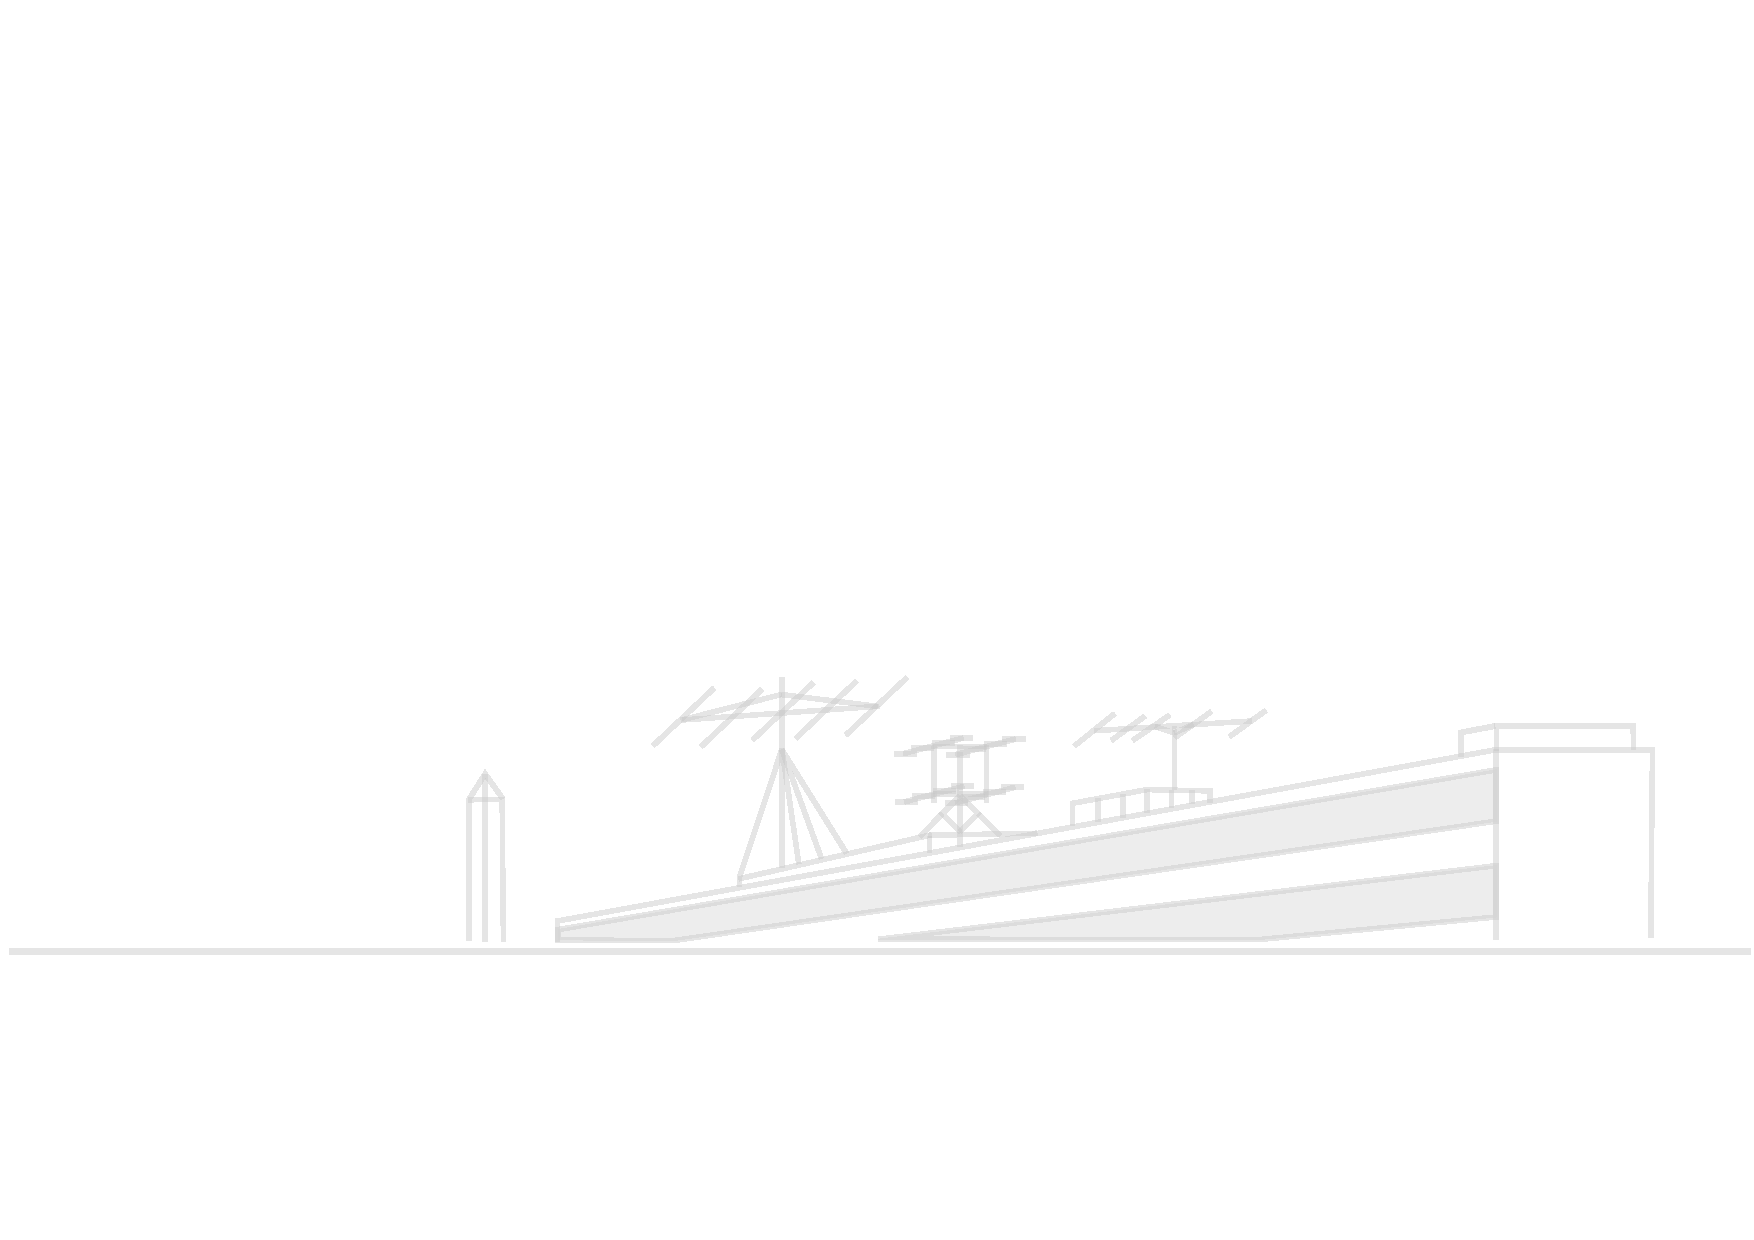
\includegraphics[width=17.8cm]{texdata/dk0tu_rooftop_background.pdf}
}

% Foliennummer einfügen
\setbeamertemplate{footline}[frame number]
%\setbeamertemplate{footline}{}

% Ändere das Zeichen vor jedem item
%\setbeamertemplate{itemize item}{\color{craneorange}$\blacktriangleright$}
%\setbeamertemplate{itemize subitem}{\color{craneorange}$\triangleright$}
%\setbeamertemplate{itemize subsubitem}{\color{craneorange}$\blacktriangleright$}

% Ändert die Blöcke 
\setbeamertemplate{blocks}[rounded][shadow=true]
% default | rounded [shadow=true|false]

%
% Eigene Kommandos
%

% Hack to get natbib and beamer working together. "The beamer user guide suggests
% that only the manual bibliography entry approach is supported"
% on some system it works out of the box, sometimes you need the hack :-(
% so check it --dl7bst
\ifdefined\newblock
    \relax
\else
    \newcommand{\newblock}{}
\fi

% \includedia command to generate png out of a dia file
% NEEDS installed dia and pdflatex option --shell-escape
\newcommand{\includedia}[1]{
    \immediate\write18{/usr/bin/dia #1.dia -e #1_diatmp.png -t png}
}

% RICHIG GROSSER FONT!
\newfont{\bigfont}{cmr10 at 144pt}
\newfont{\smallfont}{cmr10 at 8pt}

% Römische Ziffern
\makeatletter
\newcommand{\rmnum}[1]{\romannumeral #1}
\newcommand{\Rmnum}[1]{\expandafter\@slowromancap\romannumeral #1@}
\makeatother

% Schwarze Überschrift
%\setbeamercolor{frametitle}{fg=black}
%\setbeamercolor{title}{fg=black}

% Item- und Box-Farben
\definecolor{deepBlue}{HTML}{000066}
\setbeamercolor{itemize item}{fg=deepBlue}
\setbeamercolor{itemize subitem}{fg=deepBlue}
\setbeamercolor{description item}{fg=deepBlue}
\setbeamercolor{block title}{fg=deepBlue!100, bg=blue!15}
\setbeamercolor{block body}{fg=black, bg=blue!5}
\setbeamercolor{block title alerted}{fg=deepBlue, bg=red!75}
\setbeamercolor{block body alerted}{fg=black, bg=red!15}
\setbeamercolor*{block title example}{fg=blue!50, bg=blue!10}
\setbeamercolor*{block body example}{fg= blue, bg=blue!5}

%\setbeamercolor{section in head/foot}{parent=palette primary}
%\setbeamercolor{subsection in head/foot}{parent=palette secondary}
%\setbeamercolor{sidebar}{fg=darkblue,bg=yellow!90!orange}
%\setbeamercolor{title in sidebar}{fg=darkblue}
%\setbeamercolor{author in sidebar}{fg=darkblue}
%\setbeamercolor{section in sidebar}{fg=darkblue!10!black}
%\setbeamercolor{subsection in sidebar}{fg=darkblue!50!black}

% Titlepage Infos
\title{AFu-Kurs nach DJ4UF}
\author[DKØTU]{DKØTU\\ \footnotesize{Amateurfunkgruppe der TU Berlin}}
\institute[DKØTU]{\url{http://www.dk0tu.de} }

% PDF-Eigenschaften
\subject{DK0TU-Amateurfunkkurs nach DJ4UF}
\keywords{Amateurfunk Kurs HAM Radio Course CC-BY-NC-SA OpenSource TU Berlin DK0TU}

\subtitle{Technik Klasse A 03: \\
  Kondensator, Spule, Transformator \\[2em]}
\date{Stand 16.01.2017}
 \begin{document}

\begin{frame}
    \titlepage
    \vfill
    \begin{center}
        \ccbyncsaeu\\
        {\tiny This work is licensed under the \em{Creative Commons Attribution-NonCommercial-ShareAlike 3.0 License}.}\\[0.5ex]
         \tiny Amateurfunkgruppe der Technische Universität Berlin (AfuTUB), DKØTU
         %\includegraphics[scale=0.5]{img/DK0TU_Logo.pdf}
    \end{center}
\end{frame}


\section*{Einleitung}

\begin{frame}
  \frametitle{Einleitung / Kondensator}
  \begin{center}
    \Large{Wofür nutzen?}\\
    \Large{Wichtige Merkmale?}
  \end{center}
\end{frame}

\begin{frame}
  \frametitle{Einleitung / Kondensator}
  \begin{block}{Ladung und Kapazität}
    \begin{center}
      \Large{$Q = C \cdot U$}\\
      \Large{$C= \varepsilon_{0} \cdot \varepsilon_{r} \cdot \frac{A}{d}$}
    \end{center}
  \end{block}
  \begin{center}
    \begin{figure}
      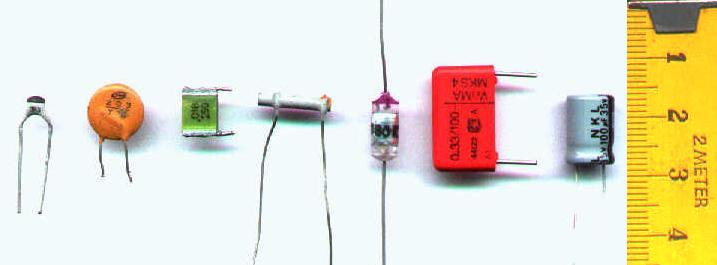
\includegraphics[width=0.9\textwidth,height=0.5\textheight,keepaspectratio]{e05/Kondensator02.jpg}
      \attribcaption{Verschiedene kleine Kondensatoren}{Aka}{https://commons.wikimedia.org/wiki/File:Condensators.JPG}{\ccbysa}
    \end{figure}
  \end{center}
\end{frame}


\begin{frame}
  \frametitle{Einleitung / Spule}
  \begin{center}
    \Large{Wofür nutzen?}\\
    \Large{Wichtige Merkmale?}
  \end{center}
\end{frame}

\begin{frame}
  \frametitle{Einleitung / Spulen-Beispiele}
  \begin{block}{Induktivität}
    \begin{center}
      \Large{$L = \cfrac{\mu_0 \cdot \mu_r \cdot N^2 \cdot A_S}{\ell_m}$}
    \end{center}
  \end{block}
  \begin{center}
    \begin{figure}
      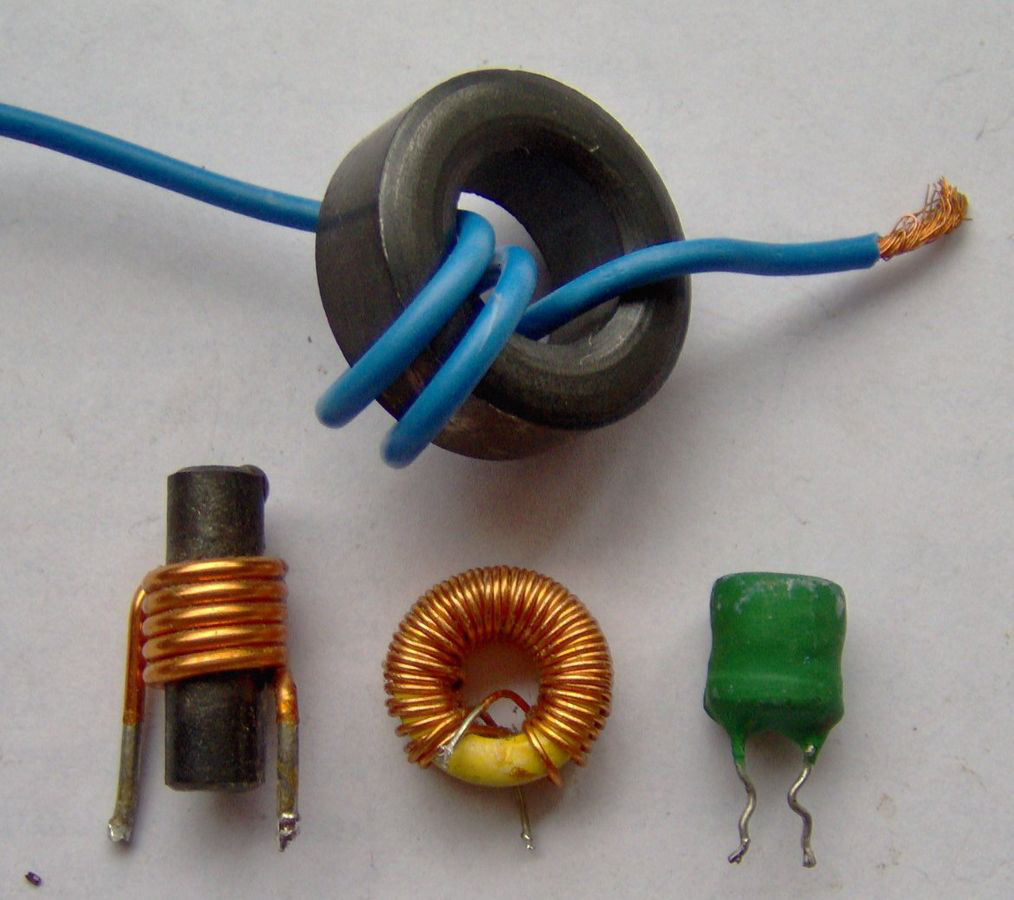
\includegraphics[width=0.6\textwidth,height=0.5\textheight,keepaspectratio]{a03/Spule.jpg}
      \attribcaption{Spulen}{FDominec}{https://commons.wikimedia.org/wiki/File:Electronic_component_inductors.jpg}{\ccbysa}
    \end{figure}
  \end{center}
\end{frame}


\section*{Laden und Entladen}

\begin{frame}
  \frametitle{Kondensator Laden}
  \begin{center}
    \Large{Mit welcher Kurve lädt sich der Kondendsator auf?}\\
  \end{center}
\end{frame}

\begin{frame}
  \frametitle{Kondensator Spannung}
  \begin{center}
    \begin{figure}
      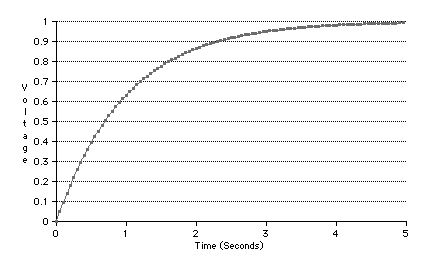
\includegraphics[width=1\textwidth,height=.75\textheight,keepaspectratio]{a03/Capacitor_Charge_Graph.jpg}
      \attribcaption{Ladevorgang eines Kondensators}{Arydberg}{https://commons.wikimedia.org/wiki/File:Capacitor_Charge_Graph.jpg}{\ccpd}
    \end{figure}
  \end{center}
\end{frame}

\begin{frame}
  \frametitle{Kondensator an Rechteckspannung}
  \begin{center}
    \begin{figure}
      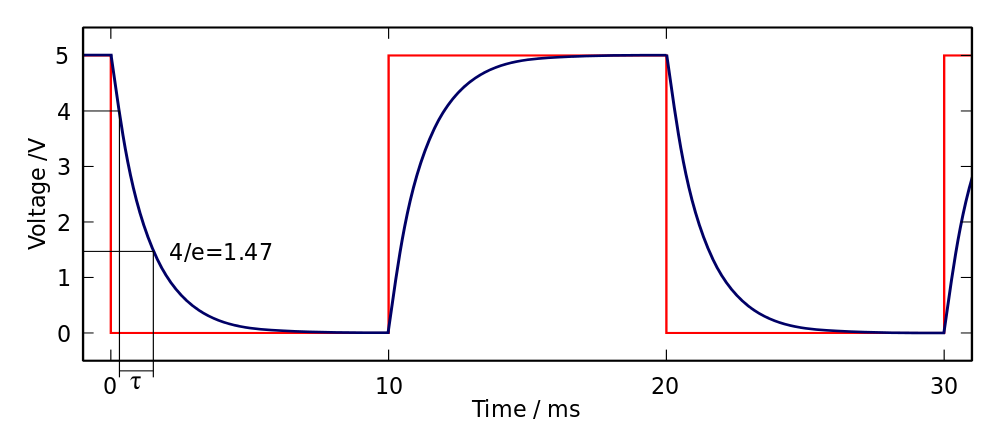
\includegraphics[width=1\textwidth,height=.75\textheight,keepaspectratio]{a03/Capacitor_Square_wave_charge-discharge.png}
      \attribcaption{Lade- und Entladevorgang eines Kondensators}{inductiveload}{https://commons.wikimedia.org/wiki/File:Capacitor_Square_wave_charge-discharge.svg}{\ccpd}
    \end{figure}
  \end{center}
\end{frame}

\begin{frame}
  \frametitle{Kondensator Strom beim Laden}
  \begin{center}
    \begin{figure}
      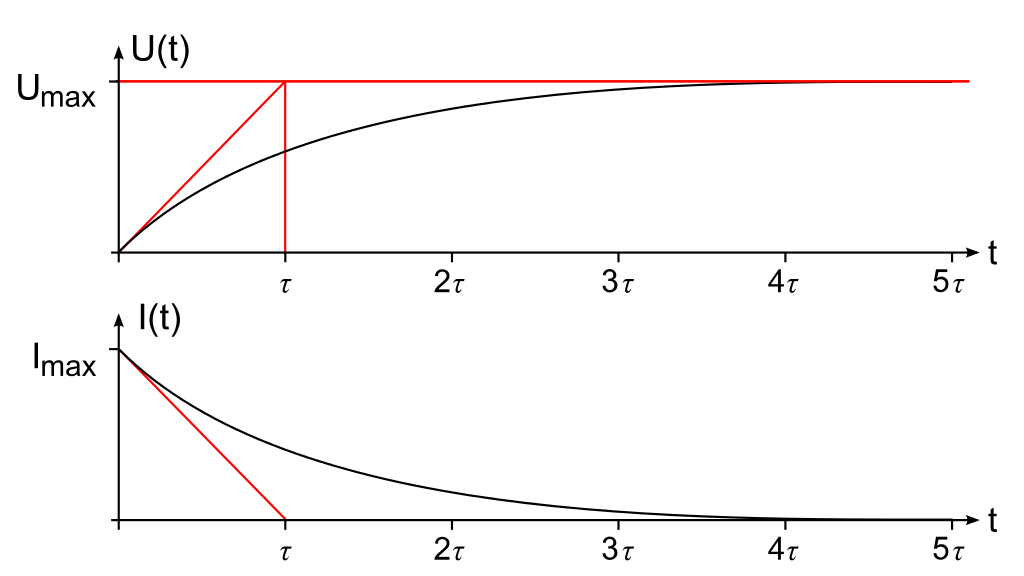
\includegraphics[width=1\textwidth,height=.6\textheight,keepaspectratio]{a03/Ladevorgang.png}
      \attribcaption{Spannung und Stromstärke bei der Kondensatorladung}{Honina}{https://commons.wikimedia.org/wiki/File:Ladevorgang.svg}{\ccpd}
    \end{figure}
    \Large{Je stärker die Spannungsänderung, desto mehr Strom fließt.}
  \end{center}
\end{frame}

\begin{frame}
  \frametitle{Kondensator Strom beim Laden}
  \begin{center}
    \begin{figure}
      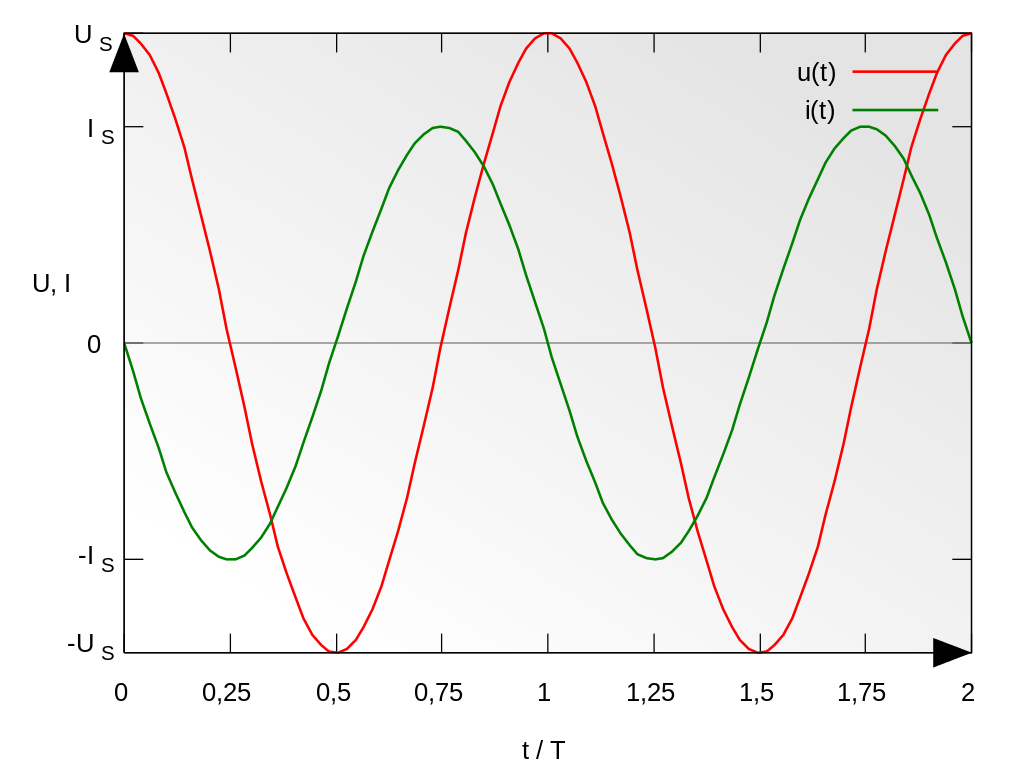
\includegraphics[width=1\textwidth,height=.75\textheight,keepaspectratio]{a03/Sinus_Voltage_and_Current_of_a_Capacitor.png}
      \attribcaption{Strom und Spannung an einem Kondensator}{Fabian R.}{https://commons.wikimedia.org/wiki/File:Sinus_Voltage_and_Current_of_a_Capacitor.svg}{\ccbysa}
    \end{figure}
  \end{center}
\end{frame}

\begin{frame}
  \frametitle{Merksatz Kondensator}
  \begin{block}{Merksatz}
    Kondensator:\\
    Strom eilt vor
  \end{block}
\end{frame}

\begin{frame}
  \frametitle{Wie verhält sich diese Schaltung?}
  \begin{center}
    \begin{figure}
      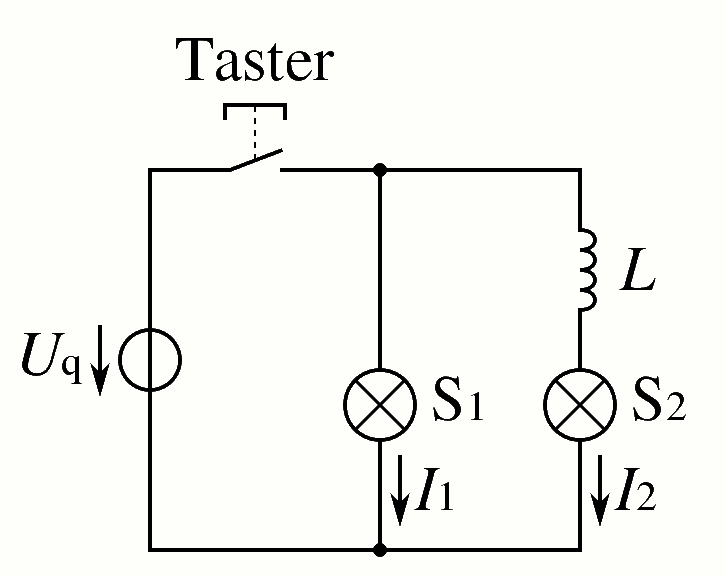
\includegraphics[width=.8\textwidth,height=.75\textheight,keepaspectratio]{a03/Spulenstrom.png}
      \attribcaption{Selbstinduktion im Gleichstromkreis (animiertes GIF)}{Stündle}{https://commons.wikimedia.org/wiki/File:Selbsti.gif}{\cczero}
    \end{figure}
  \end{center}
\end{frame}

\begin{frame}
  \frametitle{Spule}
  \begin{minipage}{0.45\textwidth}
    \begin{figure}
      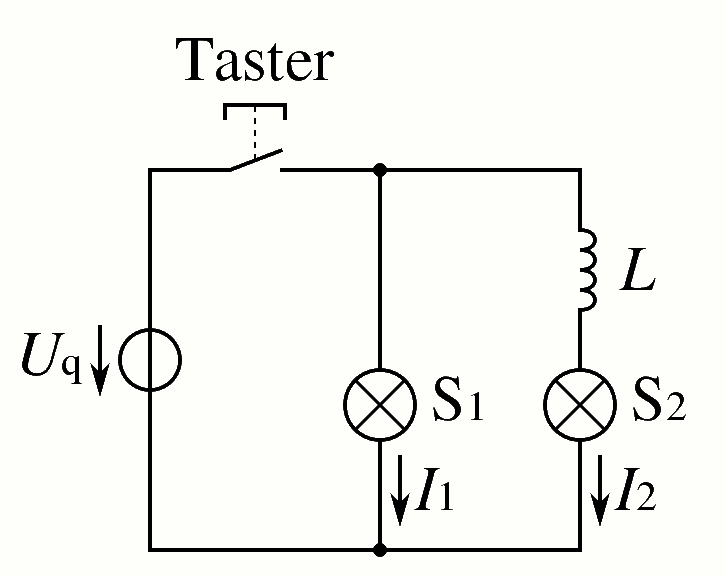
\includegraphics[width=.95\textwidth,height=.75\textheight,keepaspectratio]{a03/Spulenstrom.png}
      \attribcaption{Selbstinduktion im Gleichstromkreis (animiertes GIF)}{Stündle}{https://commons.wikimedia.org/wiki/File:Selbsti.gif}{\cczero}
    \end{figure}
  \end{minipage}
  \begin{minipage}{0.5\textwidth}
    \begin{figure}
      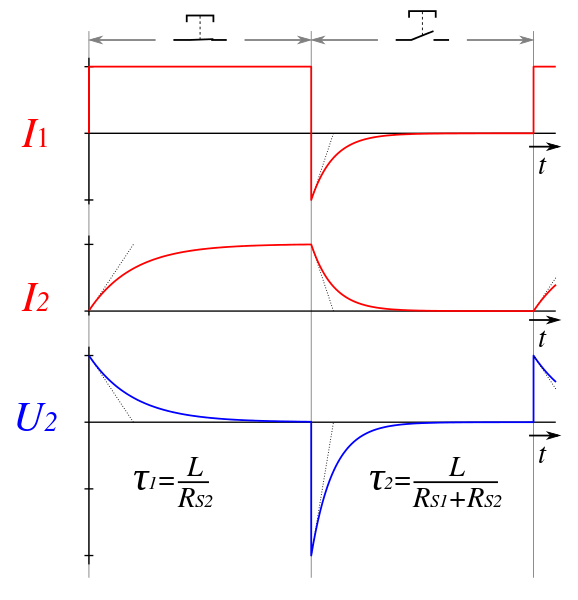
\includegraphics[width=.95\textwidth,height=.75\textheight,keepaspectratio]{a03/Selbstinduktion-im-gleichstromkreis-zeitverlauf.png}
      \attribcaption{Zeitverlauf bei der Induktion im Gleichstromkreis}{Stündle}{https://commons.wikimedia.org/wiki/File:Selbstinduktion-im-gleichstromkreis-zeitverlauf.svg}{\cczero}
    \end{figure}
  \end{minipage}
\end{frame}

\begin{frame}
  \frametitle{Phasenverschiebung Spule}
  \begin{center}
    \begin{figure}
      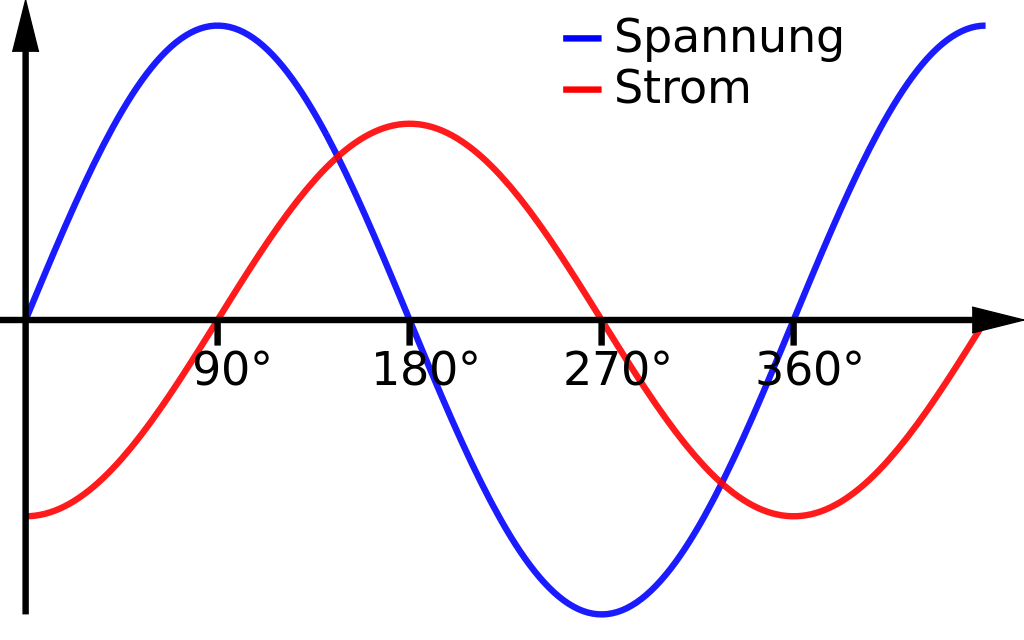
\includegraphics[width=1\textwidth,height=.75\textheight,keepaspectratio]{a03/Phasenverschiebung_induktiv.png}
      \attribcaption{Phasenverschiebung zwischen Spannung und Strom durch induktive Last}{Hyperstryke}{https://commons.wikimedia.org/wiki/File:Phasenverschiebung_induktiv.svg}{\ccpd}
    \end{figure}
  \end{center}
\end{frame}

\begin{frame}
  \frametitle{Merksatz Spule}
  \begin{block}{Merksatz}
    Bei Induktivitäten,\\
    Ströme sich verspäten.
  \end{block}
\end{frame}

\begin{frame}
  \frametitle{Merksatz Widerstand}
  \begin{block}{Merksatz}
    Beim reinen Ohmschen Widerstand\\
    gehn Strom und Spannung Hand in Hand
  \end{block}
\end{frame}

\section*{Komplexer Widerstand}

\begin{frame}
  \frametitle{Blindwiderstand}
  \begin{columns}
    \column{0.45\textwidth}
    \begin{block}{Kondensator}
      \begin{center}
        \huge{$X_{C} = \frac{1}{\omega C}$}
      \end{center}
    \end{block}

    \column{0.45\textwidth}
    \begin{block}{Spule}
      \begin{center}
        \huge{$X_{L} = \omega L$}
      \end{center}
    \end{block}
  \end{columns}

  \begin{center}
    \vspace{1cm}
    Was war nochmal $\omega$? \\
  \end{center}
\end{frame}

\begin{frame}
  \frametitle{Komplexer Widerstand}
  Für E-Techniker, aber nicht für die Amateurfunkprüfung relevant.
  \begin{center}
    \begin{figure}
      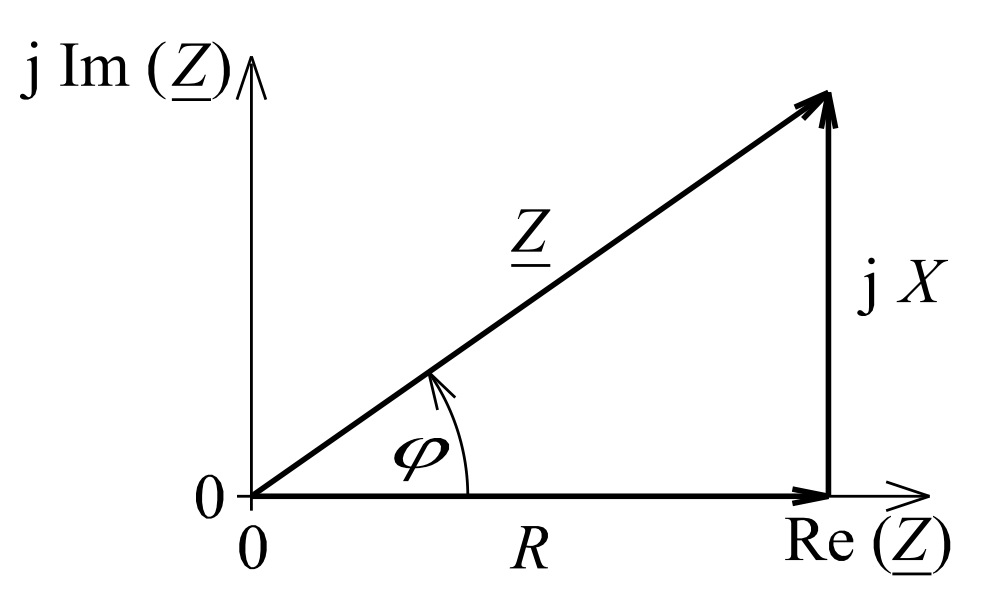
\includegraphics[width=.8\textwidth,height=.4\textheight,keepaspectratio]{a03/Widerstand_Zeiger.png}
      \attribcaption{Widerstand als Zeiger in der komplexen Ebene}{Saure}{https://commons.wikimedia.org/wiki/File:Widerstand_Zeiger.svg}{\ccbysa}
    \end{figure}
    \begin{block}{Für den Gesamtwiderstand gilt}
      $Z = R + jX$ \\
      $|Z| = \sqrt{R^2 + X^2}$
    \end{block}
  \end{center}
\end{frame}

\begin{frame}
  \frametitle{Elko Ersatzschaltbild}
  \begin{center}
    \begin{figure}
      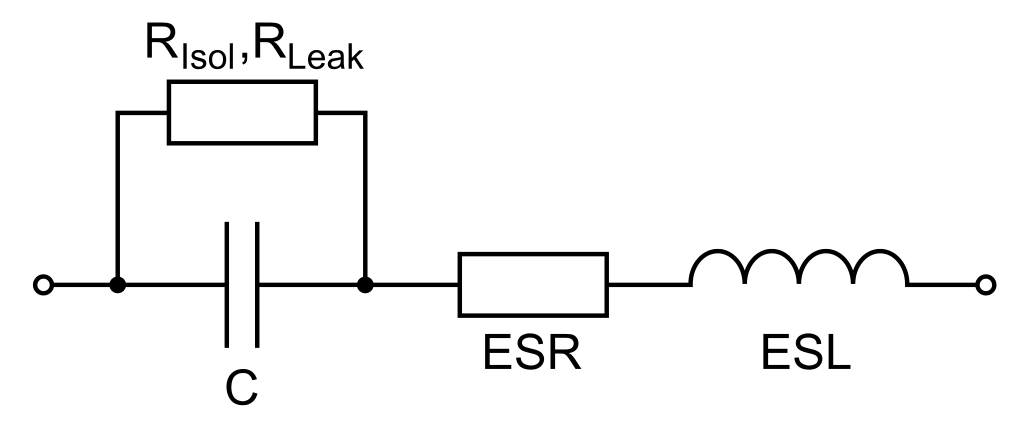
\includegraphics[width=.8\textwidth,height=.3\textheight,keepaspectratio]{a03/Elko-Ersatzschaltbild.png}
      \attribcaption{Ersatzschaltbild eines Elektrolytkondensators}{Jens Both}{https://commons.wikimedia.org/wiki/File:Widerstand_Zeiger.svg}{\ccbysa}
    \end{figure}
    nach DIN EN 60384-1 vom Februar 2002 \\[1em]

    $R_{Leak}$ $\rightarrow$ Leckströme am Elko\\
    $R_{ESR}$ $\rightarrow$ ohmsche Verluste des Bauelementes\\
    $L_{ESL}$ $\rightarrow$ Induktivität des Bauelementes\\
    Verlustfaktor $tan \delta$ $\rightarrow$ Angabe in alten Datenblättern \\im Bezug auf ESR ($\omega C \cdot$ ESR $= tan \delta$)
  \end{center}
\end{frame}


\section*{Reihen- und Parallelschaltung}

\begin{frame}
  \frametitle{Reihen- und Parallelschaltung von Kondensatoren}
  \begin{center}
    \huge Wie war noch einmal die Formel für die Reihen- und Parallelschaltung von Kondensatoren?
  \end{center}
\end{frame}

\begin{frame}
  \frametitle{Reihen- und Parallelschaltung von Kondensatoren}
  \begin{block}{Parallelschaltung von Kondensatoren}
    \begin{center}
      \huge{$C_{ges} = C_{1} + C_{2} + C_{3} + C_{4} + C_{5} + \cdots$}
    \end{center}
  \end{block}
  \pause
  \begin{block}{Reihenschaltung von Kondensatoren}
    \begin{center}
      \huge{$\frac{1}{C_{ges}} = \frac{1}{ C_{1}} + \frac{1}{C_{2}} + \frac{1}{C_{3}} + \frac{1}{C_{4}} + \frac{1}{C_{5}} + \cdots$}
    \end{center}
  \end{block}
\end{frame}

\begin{frame}
  \frametitle{Reihen- und Parallelschaltung von Spulen}
  \begin{center}
    \huge Wie war noch einmal die Formel für die Reihen- und Parallelschaltung von Spulen?
  \end{center}
\end{frame}

\begin{frame}
  \frametitle{Reihen- und Parallelschaltung von Spulen}
  \begin{block}{Reihenschaltung von Spulen}
    \begin{center}
      \huge{$L_{gesamt} = L_1 + L_2 + L_3 + \cdots$}
    \end{center}
  \end{block}
  \pause
  \begin{block}{Parallelschaltung von Spulen}
    \begin{center}
      \huge{$\frac{1}{L_{gesamt}} = \frac{1}{L_1} + \frac{1}{L_2} + \frac{1}{L_3} + \cdots$}
    \end{center}
  \end{block}
\end{frame}

\section*{Induktivitäten mit Kern}

\begin{frame}
  \frametitle{Spule mit Kern}
  \begin{center}
    Für große Induktivitäten werden die Spulen um einen Kern gewickelt.\\
    Wichtiger Wert dafür ist der Kernfaktor $A_{L}$ (immer im Datenblatt)
    \begin{block}{Induktivität von Schalenkernspulen}
      \huge $$L = N^2 \cdot A_{L}$$
    \end{block}
  \end{center}
\end{frame}

\section*{Transformator}
\begin{frame}
  \frametitle{Transformator}
  \begin{center}
    \begin{figure}
      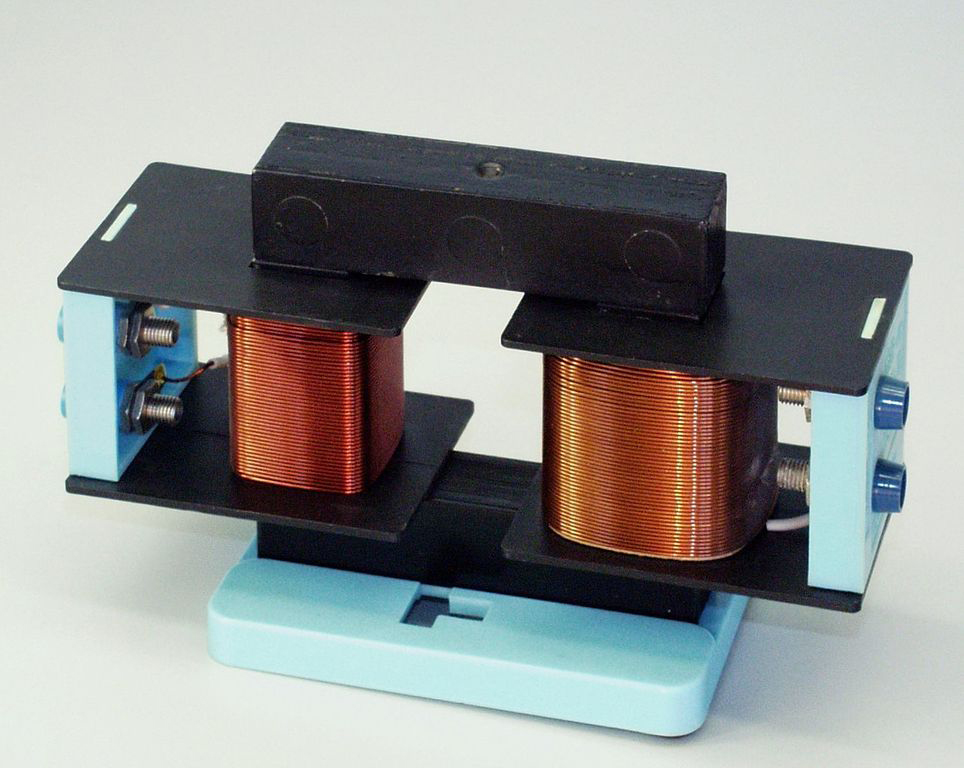
\includegraphics[width=0.9\textwidth,height=.75\textheight,keepaspectratio]{a03/trafo-Real.jpg}
      \attribcaption{Zerlegbarer Transformator für die Ausbildung}{MatthiasDD}{https://commons.wikimedia.org/wiki/File:Trafo_6.jpg}{\ccbysa}
    \end{figure}
  \end{center}
\end{frame}

\begin{frame}
  \frametitle{Transformator}
  \begin{block}{Übersetzungsverhältnis}
    $$\text{\"u} = \frac{N_P}{N_S} = \frac{U_P}{U_S} $$
  \end{block}
  \vspace{2em}
  \begin{block}{Übersetzungsverhältnis von Strom und Spannung}
    \begin{align*}
      P_P &= P_S\\
      \Rightarrow U_{P} \cdot I_P &= U_{S} \cdot I_S\\
      \Rightarrow \frac{U_P}{U_S} &= \frac{I_S}{I_P}
    \end{align*}
  \end{block}
\end{frame}

\begin{frame}
  \frametitle{Widerstandsanpassung}
  \begin{block}{Impedanzanpassung}
    $$\text{\"u} = \frac{N_P}{N_S} = \sqrt{\frac{Z_P}{Z_S}}$$
  \end{block}
  \vspace{2em}
  Wird benötigt, wenn z.B. der Fußpunktwiderstand einer Antenne bei $200\Omega$ liegt, aber mit einem $50\Omega$ Coaxkabel gespeist werden soll.
\end{frame}

\section*{Balun}

\begin{frame}
  \frametitle{Balun Theorie}
  \begin{center}
    \begin{figure}
      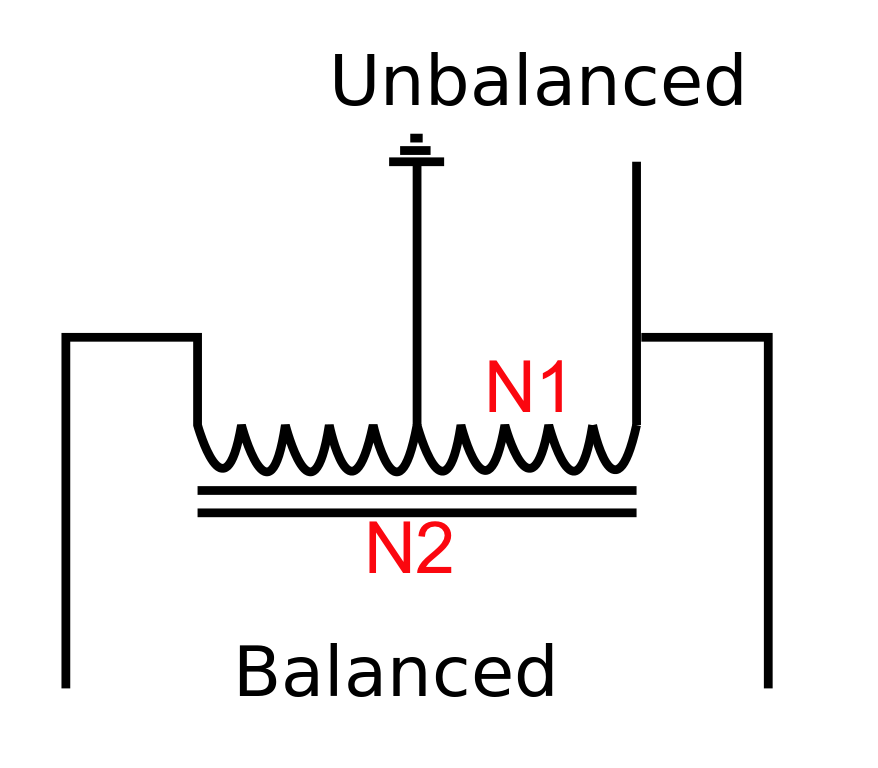
\includegraphics[width=0.8\textwidth,height=.75\textheight,keepaspectratio]{a03/Cdbalun2.png}
      \attribcaption{Balun (schematisch)}{Wolfmankurd}{https://commons.wikimedia.org/wiki/File:Cdbalun2.svg}{\ccbysa}
    \end{figure}
  \end{center}
\end{frame}

\begin{frame}
  \frametitle{Balun Real}
  \begin{center}
    \begin{figure}
      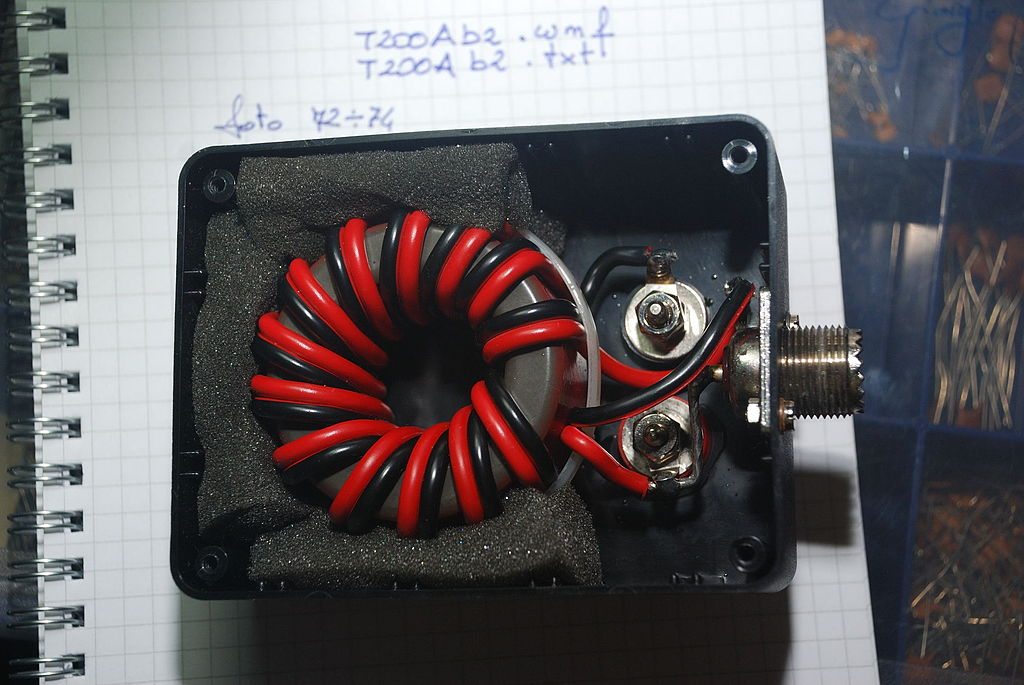
\includegraphics[width=0.9\textwidth,height=.75\textheight,keepaspectratio]{a03/balun-Real.jpg}
      \attribcaption{Balun 4:1, 13 turns on T200A/2}{Giorgio Brida}{https://commons.wikimedia.org/wiki/File:T200A2.jpg}{\ccby}
    \end{figure}
  \end{center}
\end{frame}


\renewcommand{\refname}{Referenzen}

\hypertarget{refs}{}
\textcolor{white}{} \\ %\vspace{} geht nicht
\Large Referenzen/Links
\footnotesize

\begin{thebibliography}{}
  \bibitem{dj4uf} Moltrecht A 03: \\
    \url{https://www.darc.de/der-club/referate/ajw/lehrgang-ta/a03/}

\end{thebibliography}

% Hier könnte noch eine Kontaktfolie stehen

\end{document}

